(Gusfield Chapter 1)

\section{Speeding Up the Naive Algorithm}

The naive exact matching algorithm is stupid. It always shifts $P$ by only one even if it knows for sure that the next shift will not yield a match. This gives us some ideas on how to improve the algorithm. If we can shift $P$ by more than one character, but never shift so far as to miss the next occurrence of $P$ in $T$, we can improve the runtime of the naive algorithm.

Doing this, however, requires us to have some prior knowledge of the pattern $P$ or the text $T$.

\section{Foundamental Preprocessing}

A fundemental preprocessing is a generalized way to process the pattern $P$ to gain knowledge of the pattern, independent of any particular algorithm.

\begin{definition}
    Given a string $S$ and a position $i>1$, let $Z_i(S)$ be the length of the longest substring of $S$ that starts at $i$ and matches a prefix of $S$.

    In other words, $Z_i(S)$ is the length of the longest prefix of $S[i\ldots |S|]$ that matches a prefix of $S$.
\end{definition}

\begin{definition}[Z-box] \index{Z-box}
    For any position $i > 1$ where $Z_i$ is greater than 0, the \textbf{Z-box} at $i$ is the interval starting at $i$ and ending at $i+Z_i-1$.
\end{definition}

\begin{marginfigure}
    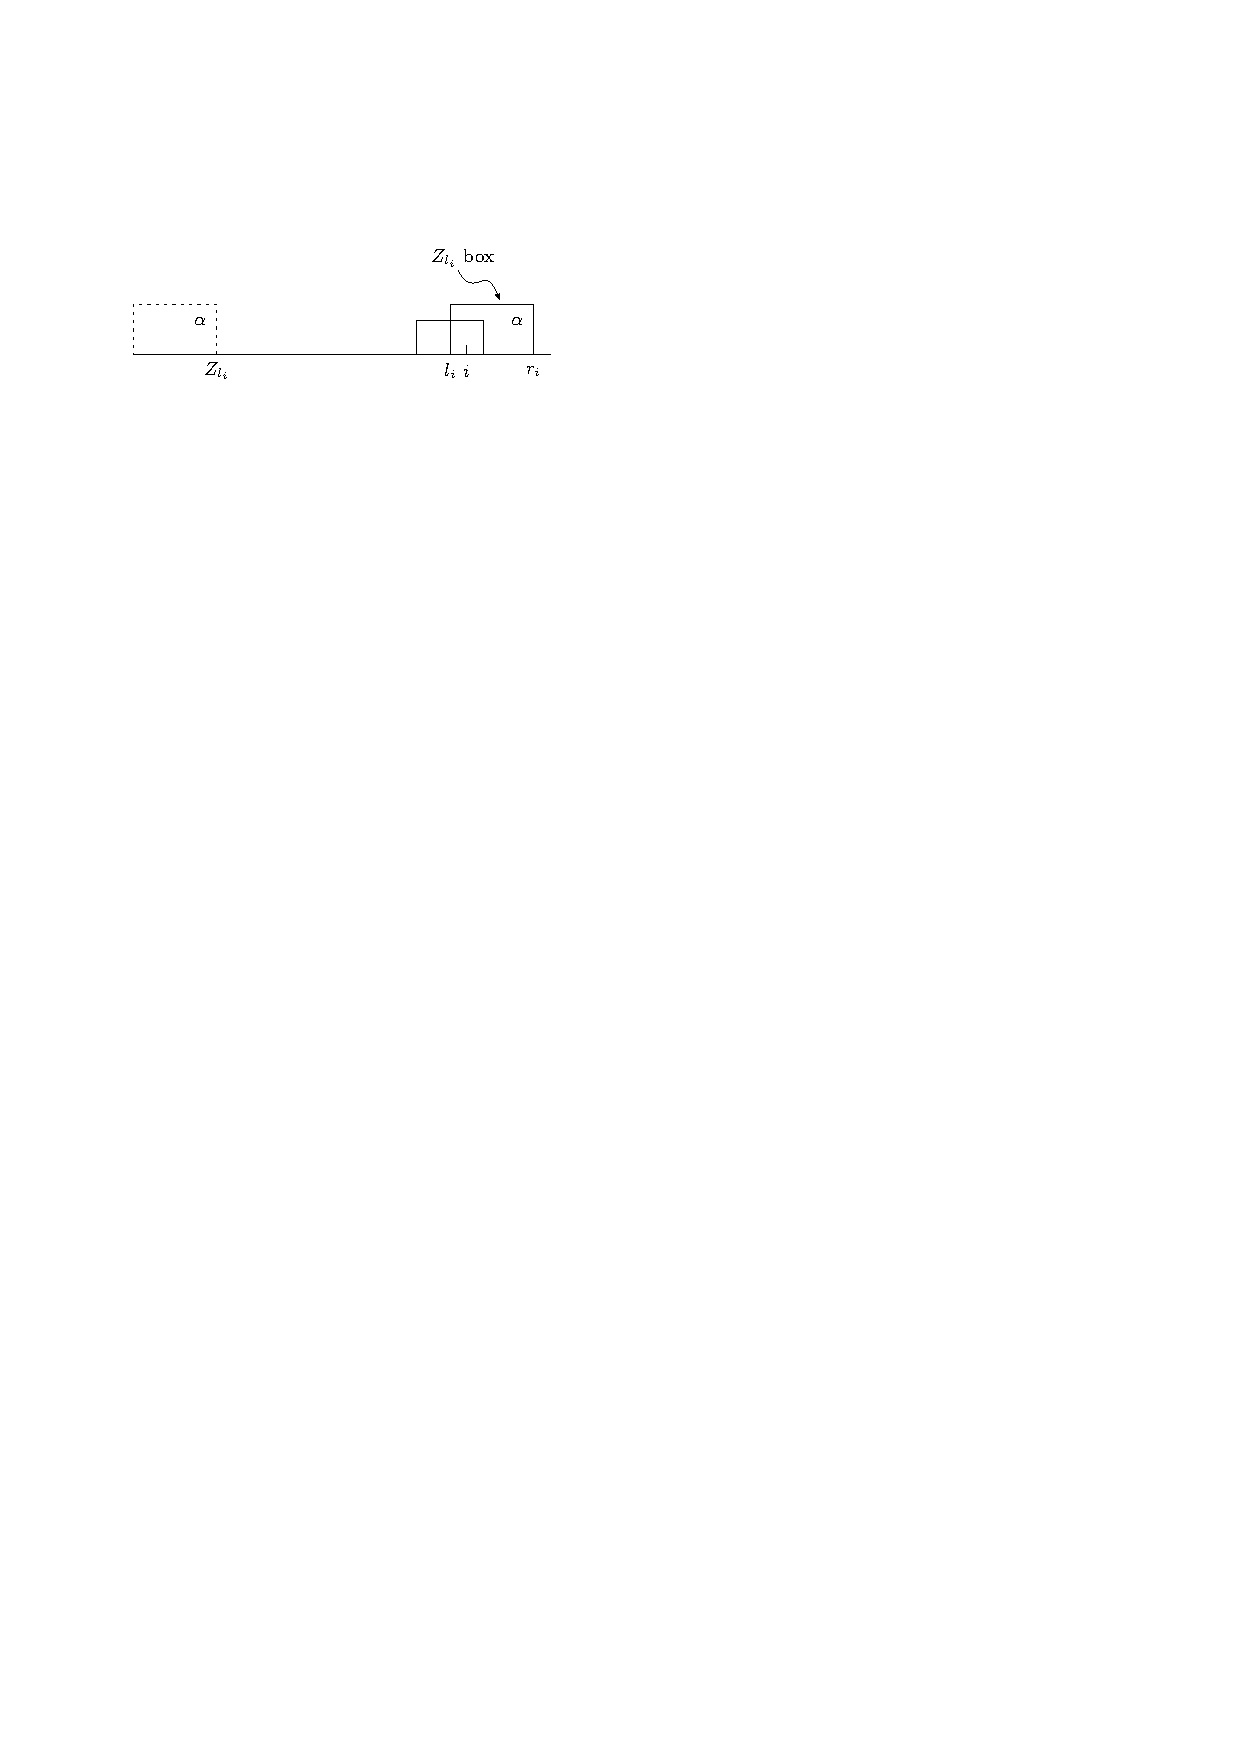
\includegraphics[width=\linewidth]{z/z-box.pdf}
    \caption{Relations between $i$, $l_i$, $r_i$ and the Z-box at $l_i$.}
    \label{fig:z-box}
\end{marginfigure}

\begin{definition}
    For every $i > 1$, $r_i$ is the right endpoint of the Z-box that begins at or befor position $i$ (i.e. the closest Z-box to the left). More formally, $r_i$ is the largest value of $j + Z_j - 1$ over all $1 < j \leq i$ such that $Z_j > 0$.
\end{definition}

\index{fundamental preprocessing}
The linear-time computation of the $Z_i$ values for all $i \in \{1,\ldots,|S|\}$ from the string $S$ is called the \textit{\textbf{fundamental preprocessing}} task.

\section{The Z Algorithm} \index{Z algorithm}

The \textit{\textbf{Z algorithm}} is an algorithm for computing the fundamental preprocessing. The Z algorithm is similar to a dynamic programming algorithm in the sense that it uses memoized information to speed up the computation and reduce the number of comparison needed. Namely, assume there exists $j < i$ such that $j + Z[j] - 1 > i$, then we can use $Z[i-j+1]$ to infer $Z[i]$.

\begin{figure}[htbp]
    \centering
    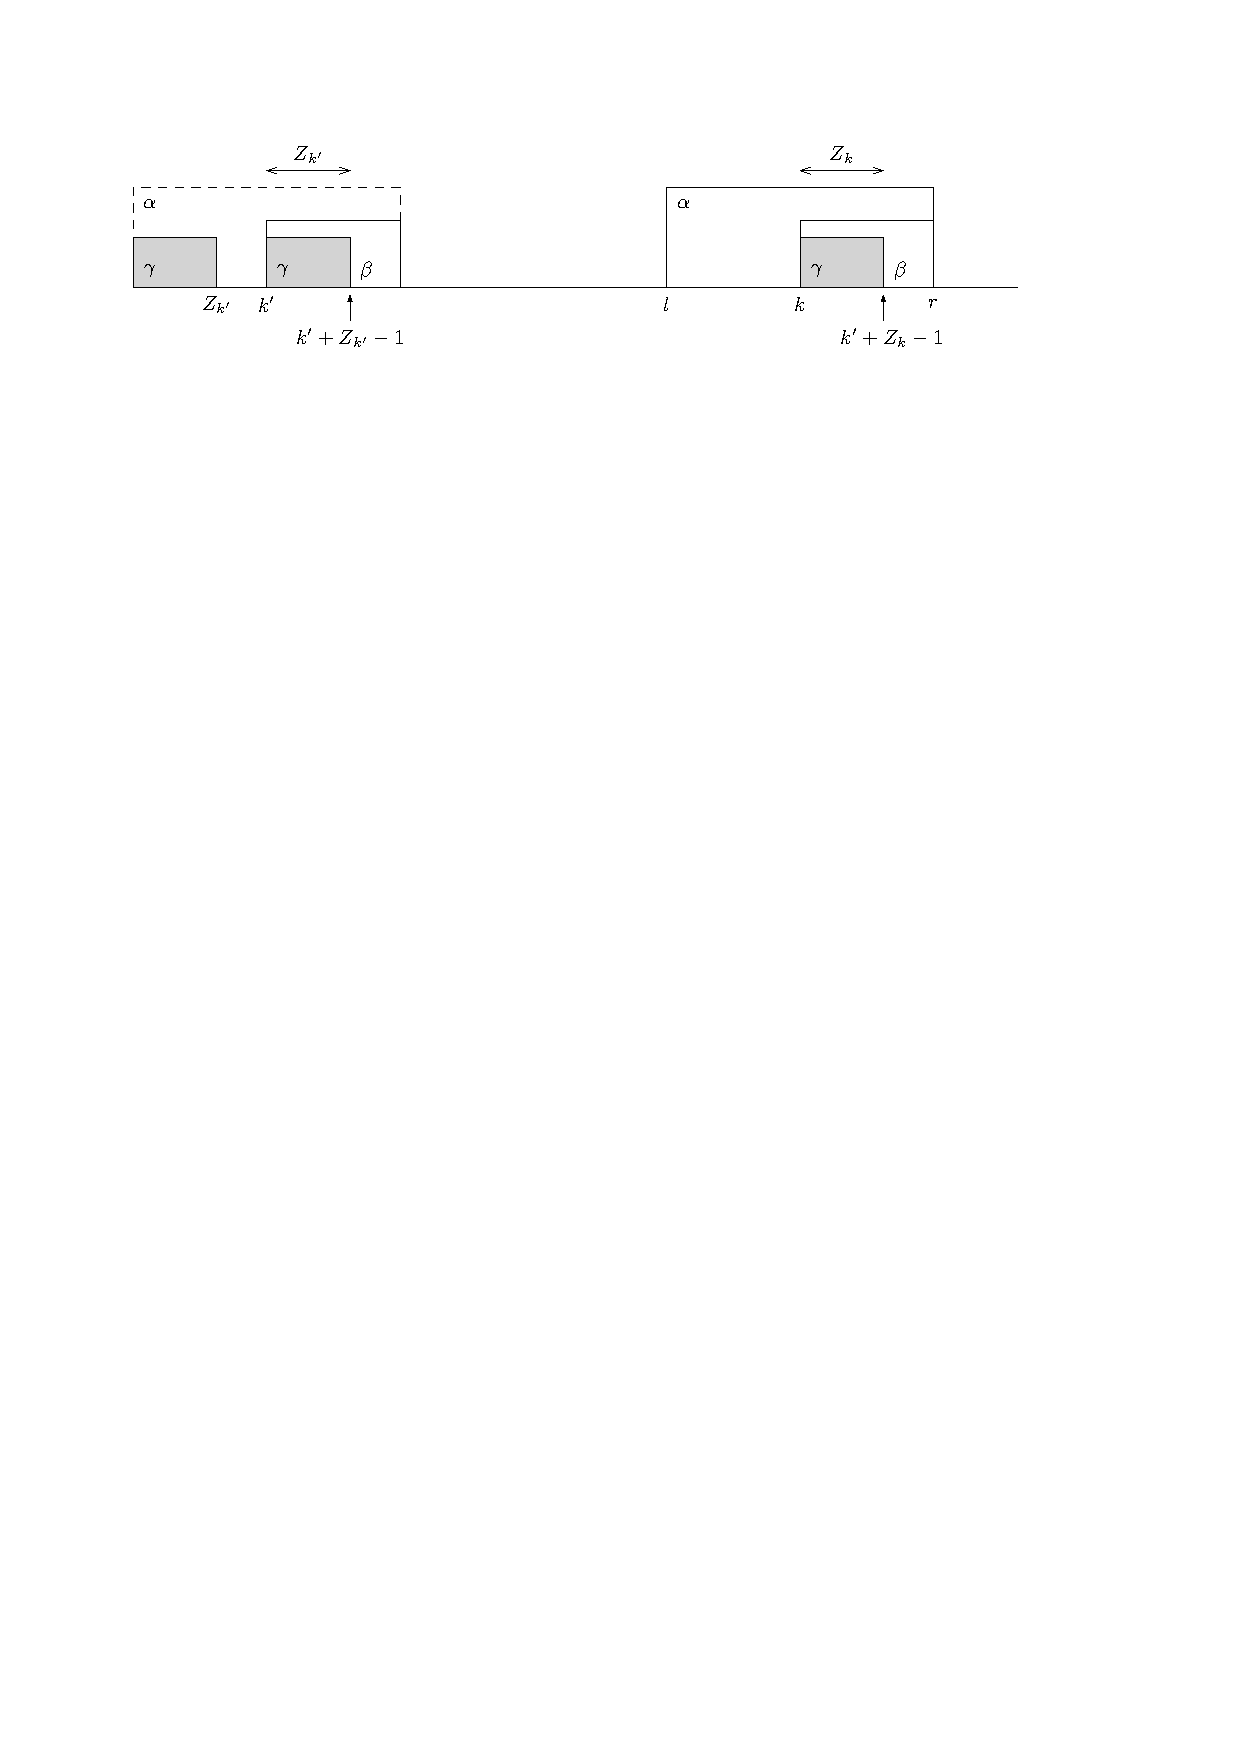
\includegraphics[width=\linewidth]{z/z-process-case2a.pdf}
    \caption{Case 2a: The longest string starting at $k'$ that matches a prefix of $S$ is shorter than $|\beta| = r-k+1$. In this case, $Z_k = Z_{k'}$.}
    \label{fig:z-process-case2a}
\end{figure}

\begin{figure}[htbp]
    \centering
    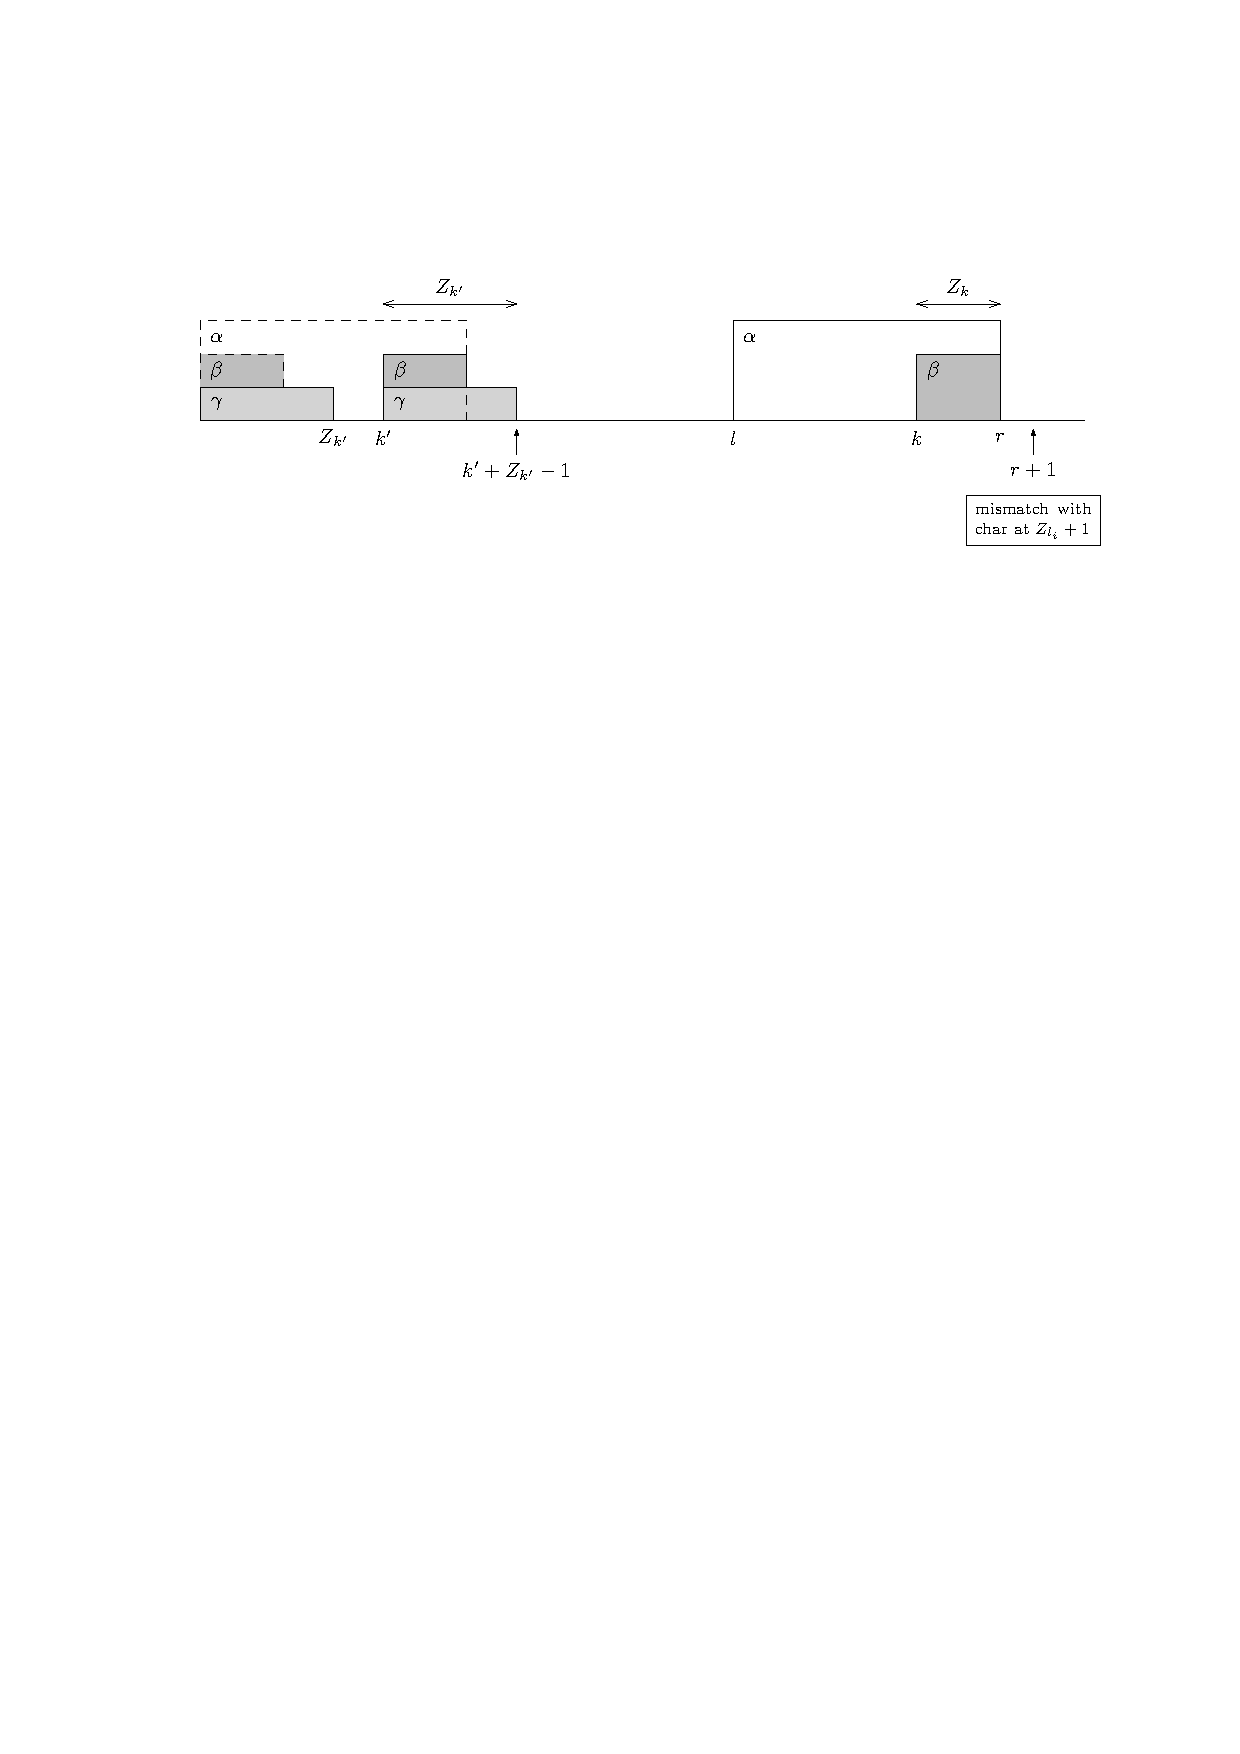
\includegraphics[width=\linewidth]{z/z-process-case2b1.pdf}
    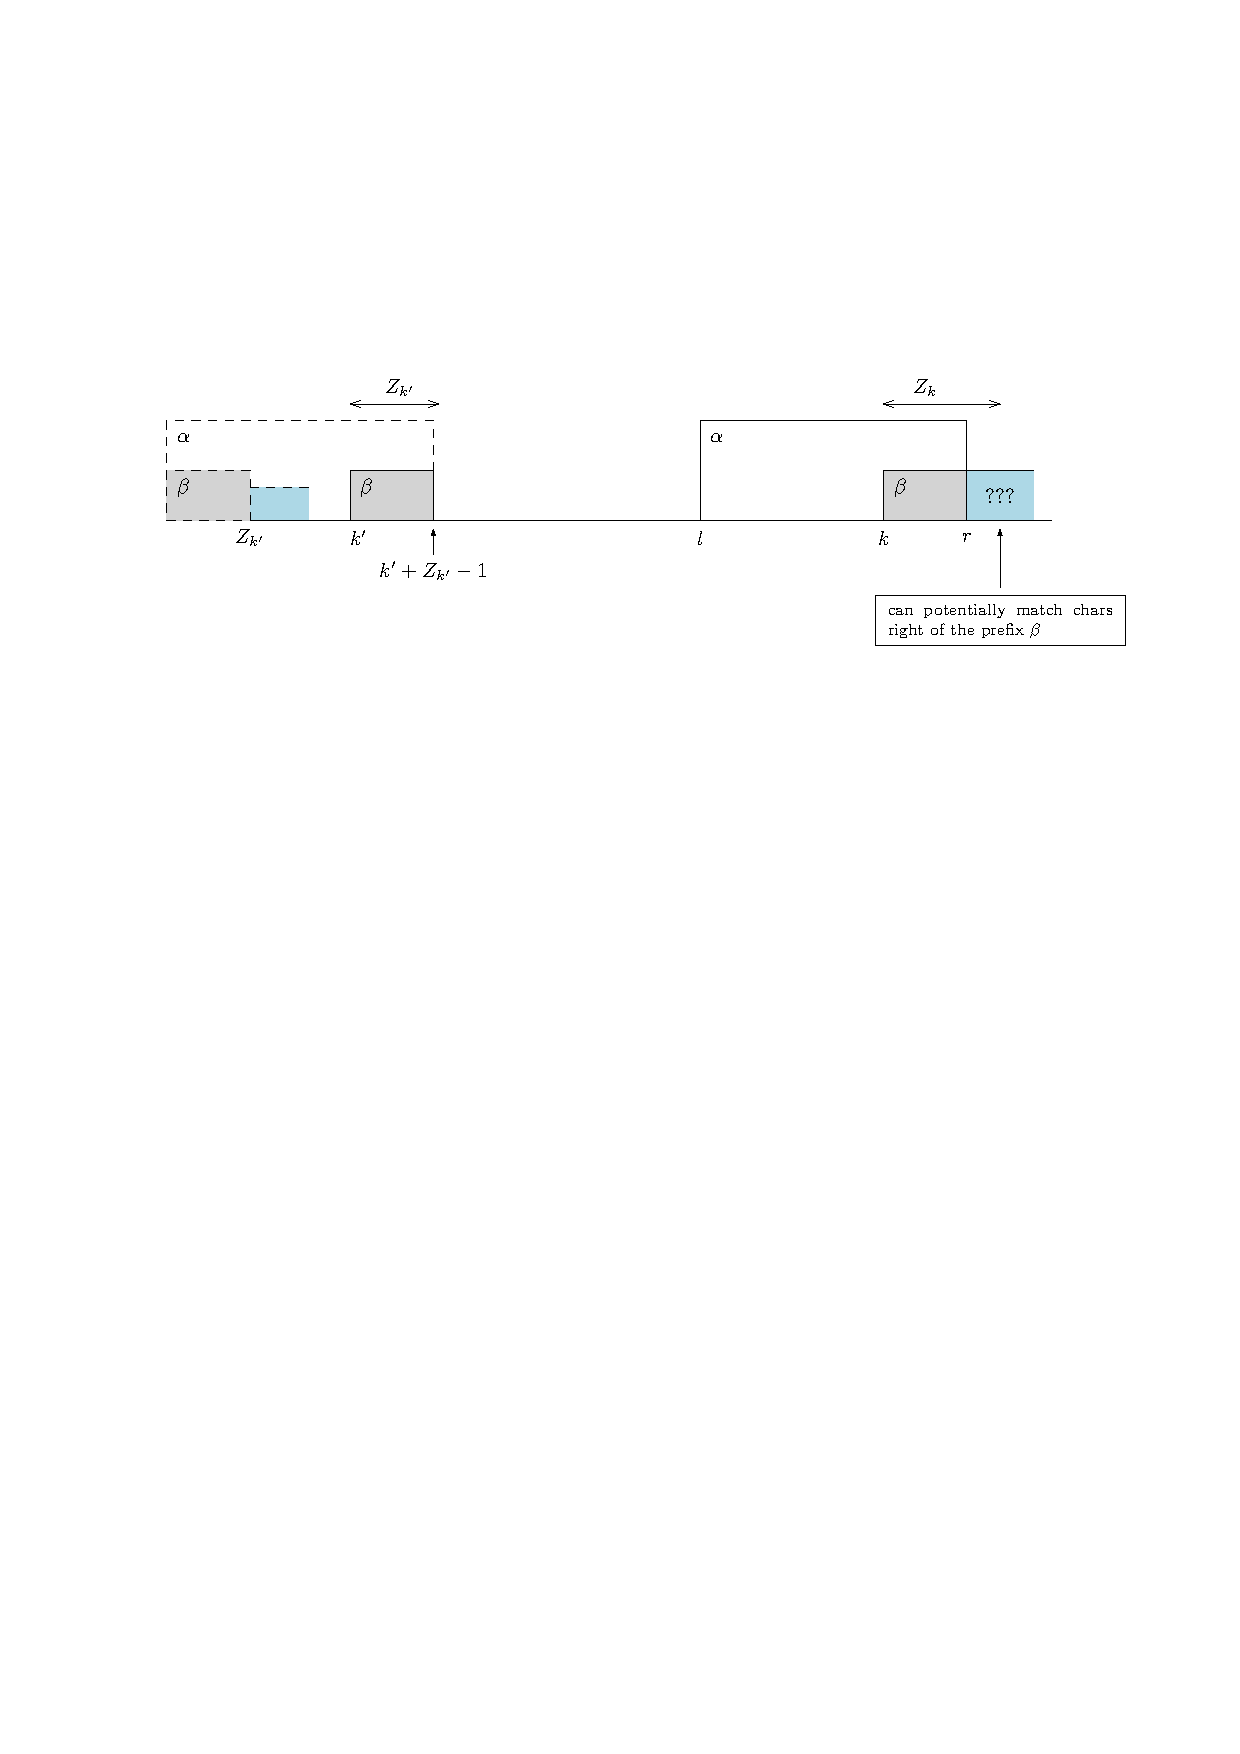
\includegraphics[width=\linewidth]{z/z-process-case2b2.pdf}
    \caption{Case 2b: The longest string starting at $k'$ that matches a prefix of $S$ is at least $|\beta| = r-k+1$. In this case, we continue to compare characters right of $r$ with characters right of the $Z_{k'}$th character until mismatch. }
    \label{fig:z-process-case2b}
\end{figure}

Given $Z_i$ for all $1 < i \leq k-1$ and the current $l$ and $r$, we can compute $Z_k$ using the following procedure:

\begin{enumerate}
    \item Case 1: If $k > r$, $k$ is not in an existing Z-box. Compute $Z_k$ by explicitly comparing each character starting at $k$ with prefix of $S$.
    \item Case 2: If $k \leq r$, $k$ is in an existing Z-box, denoted $\alpha$, that matches a prefix of $S$. Hence, character $S[k]$ also appears in the prefix at position $k' = k - l + 1$. \\ We also consider the substring $S[k\ldots r]$, denoted $\beta$. By the same reasoning, $\beta$ matches the substring $S[k'\ldots Z_l]$.
    \begin{enumerate}
        \item $Z_{k'} < |\beta|$. This implies that the longest string starting at $k'$ that matches a prefix of $S$, $\gamma$, is shorter $|\beta|$. Then, $Z_{k} = Z_{k'}$, and $l,r$ remain unchanged. Note that $|\gamma|$ can be 0.
        \item $Z_{k'} \geq |\beta|$. This means $S[k\ldots r]$ is at least a prefix of $S$. However, $Z_k$ might be larger than $|\beta|$. We cannot determine this solely based on the existing information as characters beyond the $Z_l$th character are not included in $\alpha$. So, we compare the characters starting at position $r+1$ of $S$ to the characters starting at position $|\beta|+1$ of $S$, until a mismatch occurs. Say the mismatch occur at position $q$. Then, $Z_k = q- k$, $r = q-1$, and $l = k$. (If $Z_{k'} > |\beta|$, a mismatch occurs immediate after the $Z_{l}$th character because otherwise, the $(r+1)$th character matches the $Z_{l}$th character, and we would have a longer $\alpha$ and a larger $Z_l$)
    \end{enumerate}
\end{enumerate}

\begin{codebox}
    \Procname{$\proc{Compute-Z}(S)$}
    \li $n = |S|$
    \li $l,r,k = 1$
    \li $Z = \text{empty array of length $n$}$
    \li \For $k=2$ \To $n$ \Do
        \li \If $k > r$ \Then \RComment{Case 1}
            \li \Comment{compute $Z[k]$ from scratch}
            \li $l,r = k$ 
            \li \While $r \leq n$ \textbf{and} $S[r-l+1] \isequal S[r]$ \Do
                \li $r = r + 1$
            \End
            \li $Z[k] = r-l$
            \li $r = r - 1$
        \li \Else \RComment{Case 2}
            \li $k' = k - l + 1$
            \li \If $Z[k'] < r - k + 1$ \Then \RComment{Case 2a}
                \li $Z[k] = Z[k']$ 
            \li \Else \RComment{Case 2b}
                \li $q = r+1$
                \li \While $q \leq n$ \textbf{and} $S[q-l + 1] \isequal S[q]$ \Do
                    \li $q = q + 1$
                \End
                \li $Z[k] = q-k$
                \li $l,r = k, \,q-1$ 
            \End
        \End
        \End
        \li \Return $Z$ 
\end{codebox}

For a step-by-step animation of the Z algorithm, see \\
\href{https://personal.utdallas.edu/~besp/demo/John2010/z-algorithm.htm}{https://personal.utdallas.edu/\textasciitilde besp/demo/John2010/z-algorithm.htm}

\section{Running Time of the Z Algorithm}

\begin{theorem}
    All the $Z_i$ values can be computed by the Z algorithm with at most $2|S| \in O(|S|)$ comparisons.
\end{theorem}

\begin{proof}
    The time is proportional to the number of iterations, $|S|$, plus the number of character comparisons.
    
    Each iteration that does any character comparison ends as soon as there is a mismatch, so there are at most $|S|$ \textbf{mismatches}. In every iteration where there is a match, $r$ moves to the right by an amount at least as large as the number of matches. This implies that there are at most $|S|$ \textbf{matches}. Note that once a character results in a match, it is not compared again.

    Every character comparison is either a match or mismatch, so the total number of comparisons is at most $2|S|$.
\end{proof}

\section{Correctness of the Z Algorithm}

\begin{theorem}
    At the $k$th iteration of the algorithm, \proc{Compute-Z} correctly calculates $Z_k$, and $l,r$ are updated correctly.
\end{theorem}

\begin{proof}
    By a case analysis.

    Case 1: Trivial since it's just explicit comparison.

    Case 2a: We claim that the substring at position $k$ can match a prefix of $S$ only for length $Z_{k'} < |\beta|$. Prove the claim by contradiction (suppose not, we would have a longer prefix matching the substring at $k'$, contradicting the maximality of $Z_{k'}$).

    Case 2b: $\beta$ must be a prefix of $S$ as established above. Characters beyond $r$ are explicitly compared.
\end{proof}

\begin{corollary}
    \proc{Compute-Z} correctly calculates $Z_k$ for all $k \in \{2,\ldots,|S|\}$.
\end{corollary}

\begin{proof}
    By induction on $k$.
\end{proof}

\section{Z Algorithm for Exact Matching}

The Z algorithm lends itself to a linear-time algorithm for exact matching. Given a pattern $P$ and text $T$, we construct a new string $P \$ T$ where $\$$ is a \textit{\textbf{separator}} (a.k.a. \textit{\textbf{delimiter}} or \textit{\textbf{sentinel}}) such that $\$ \not\in \Sigma$. We construct the Z-array for this new string. It takes $O(|P|+|T|)$ time to construct the Z-array. After this, we can simply make a pass through the Z-array and read the result from it. This takes $O(|T|)$ time.

\begin{codebox}
    \Procname{$\proc{Z-Exact-Matching}(P,T)$}
    \li $\id{query} = P + ``\$" + T$
    \li $Z = \proc{Compute-Z}(\id{query})$
    \li \For $i = |P|+1$ \To $|P|+|T|+1$ \Do
        \li \If $Z[i] \isequal |P|$ \Then
            \li pattern found at index $i - |P|$ 
\end{codebox}